% editing notes: don't use auto-fill-mode

\documentclass[man,floatsintext]{apa6}
\usepackage{longtable}
\usepackage{amsmath}
\usepackage{amssymb}
\usepackage{graphicx}
% \usepackage{geometry}
\usepackage{hyperref}
\usepackage[natbibapa]{apacite}
\usepackage{times}
\usepackage{multirow}
\usepackage{color}
\usepackage{array}
\usepackage{verbatim}

\newcommand{\tcite}[1]{$\langle${\footnotesize \texttt{#1}}$\rangle$}

\newcommand{\cas}[1]{ {\color{blue}  #1} }

\graphicspath{{images/}}

\shorttitle{Semantic coherence and distributional learning}
% \shorttitle{}
\title{Semantic coherence facilitates distributional learning}
\author{Long Ouyang, Lera Boroditsky, Michael C. Frank}
\affiliation{Department of Psychology, Stanford University\vskip 5em Word count: 8,298}

\authornote{An earlier version of this paper appeared in the Proceedings of the 34th Annual Meeting of the Cognitive Science Society. Address correspondence to:\\
  Long Ouyang~\\
  Jordan Hall, Building 01-420\\
  450 Serra Mall\\
  Stanford, CA, 94305\\
  Email: \texttt{longouyang@post.harvard.edu}}

\abstract{
  Computational models have shown that purely statistical knowledge about words' linguistic contexts is sufficient to learn many properties of words, including syntactic and semantic category.
  For example, models can infer that ``postman'' and ``mailman'' are semantically similar because they have quantitatively similar patterns of association with \emph{other} words (e.g., they both tend to occur with words like ``deliver'', ``truck'', ``package'').
  Contra these computational results, artificial language learning experiments suggest that distributional statistics \emph{alone} do not facilitate learning of linguistic categories.
  However, experiments in this paradigm expose participants to entirely novel words, whereas real language learners encounter input that contains some known words that are semantically organized.
  In three experiments, we show that (1) the presence of familiar semantic reference points facilitates distributional learning and (2) this effect crucially depends both on the presence of known words and the adherence of these known words to some semantic organization.
}

\keywords{distributional learning; word learning; semantic coherence}

\begin{document}
\maketitle
\input{main.tex}
\newpage
\bibliographystyle{apacite}
\bibliography{references}
\section{Old versus new stimuli comparison}
\label{old-vs-new}

We performed a partial replication of Experiment 1a with the new stimuli. We collected data in four out of the sixteen experimental conditions and the results mirror those found with the old stimuli:

\begin{center}
  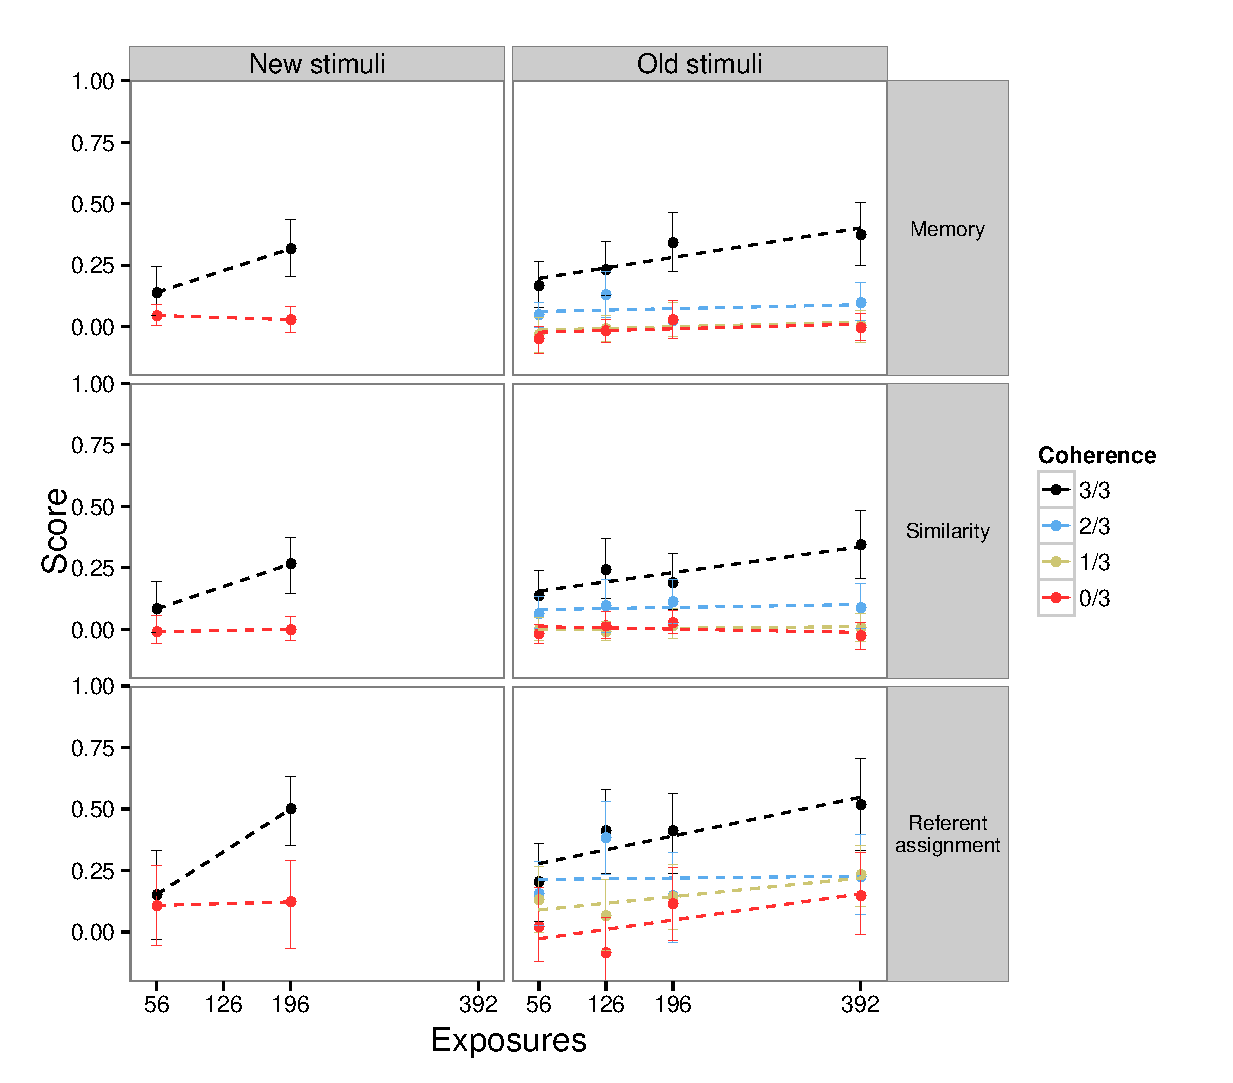
\includegraphics[width=0.9\linewidth]{stim-comparison} \\

\end{center}
\section{$t$-tests for familiarity orderings in the memory task}
\begin{figure}[h]
  \begin{center}
    \begin{tabular}{ c c}

      \textbf{0/3 coherence}: df = 150 & \textbf{1/3 coherence}: df = 153\\

      {
        % -------------- none --------------
        % df = 150

        % Pairwise comparisons using paired t tests

        % data:  e$mem.score and e$type

        % familiar withheld cross
        % withheld 0.01266  -        -
        % cross    0.06278  0.48454  -
        % position 0.00029  0.21723  0.08529

        % P value adjustment method: holm
      \small

      \begin{tabular}{| l | l |  l | l |}
        \hline
        & F              & W           & C \\
        \hline
        W & $p$ = 0.01*  &             &\\
        \hline
        C & $p$ = 0.06 &  $p$ = 0.48 & \\
        \hline
        P & $p$ $<$ 0.001* &  $p$ = 0.21 &  $p$ = 0.08 \\
        \hline
      \end{tabular}
      } &

          {
            % -------------- sem1 --------------
            % df = 153

            % Pairwise comparisons using paired t tests

            % data:  e$mem.score and e$type

            % familiar withheld cross
            % withheld 7.4e-08  -        -
            % cross    3.8e-06  0.525    -
            % position 2.1e-12  0.085    0.018

          \small
          \begin{tabular}{| l | l |  l | l |}
            \hline
            & F               & W           & C \\
            \hline
            W &  $p$ $<$ 0.001* &             &\\
            \hline
            C &  $p$ $<$ 0.001* &  $p$ = 0.52 &\\
            \hline
            P &  $p$ $<$ 0.001* &  $p$ = 0.08 &  $p$ = 0.01*\\
            \hline
          \end{tabular}
      }\\

      \textbf{2/3 coherence}: df = 164 & \textbf{3/3 coherence}: df = 152\\

      {

        % -------------- sem2 --------------
        % df = 164

        % Pairwise comparisons using paired t tests

        % data:  e$mem.score and e$type

        % familiar withheld cross
        % withheld 1.2e-05  -        -
        % cross    4.0e-14  0.00056  -
        % position $<$ 2e-16  3.5e-11  0.00056

        % P value adjustment method: holm


      \small
      \begin{tabular}{| l | l |  l | l |}
        \hline
        & F                           & W                         & C \\
        \hline
        W &  $p$ $<$ 0.001*  &                           &\\
        \hline
        C &  $p$ $<$ 0.001*  &  $p$ $<$ 0.001*  &\\
        \hline
        P &  $p$ $<$ 0.001* &  $p$ $<$ 0.001*  &  $p$ $<$ 0.001*\\
        \hline
      \end{tabular}
      } &

          {

            % -------------- sem3 --------------
            % df = 152

            % Pairwise comparisons using paired t tests

            % data:  e$mem.score and e$type

            % familiar withheld cross
            % withheld 0.00016  -        -
            % cross    4.4e-16  4.4e-16  -
            % position $<$ 2e-16  $<$ 2e-16  4.4e-16

            % P value adjustment method: holm

          \small
          \begin{tabular}{| l | l |  l | l |}
            \hline
            & F                            & W                         & C \\
            \hline
            W &  $p$ $<$ 0.001*  &                           &\\
            \hline
            C &  $p$ $<$ 0.001*  &  $p$ $<$ 0.001*   &\\
            \hline
            P &  $p$ $<$ 0.001* &  $p$ $<$ 0.001*  &  $p$ $<$ 0.001*\\
            \hline
          \end{tabular}
      }\\
      \textbf{Nonce 3/3 coherence}: df = 150 & \\
      {
        % -------------- nc-sem3 --------------
        % df = 150

        % Pairwise comparisons using paired t tests

        % data:  e$mem.score and e$type

        % familiar withheld cross
        % withheld 0.53     -        -
        % cross    $<$ 2e-16  5.4e-14  -
        % position $<$ 2e-16  $<$ 2e-16  $<$ 2e-16

        % P value adjustment method: holm

      \small
      \begin{tabular}{| l | l |  l | l |}
        \hline
        & F                            & W                         & C \\
        \hline
        W &  $p$ $<$ 0.53  &                           &\\
        \hline
        C &  $p$ $<$ 0.001*  &  $p$ $<$ 0.001*   &\\
        \hline
        P &  $p$ $<$ 0.001* &  $p$ $<$ 0.001*  &  $p$ $<$ 0.001*\\
        \hline
      \end{tabular}
      } & \\

    \end{tabular}
    \caption{$p$ values for paired-sample t-tests of familiarity ratings for (F)amiliar, (W)ithheld, (C)o-occurrence violation, and (P)osition violation sentences in Experiments 1a and 1b. $p$ values have been adjusted for multiple comparisons using the Holm procedure.}
    \label{familiarity-ordering-t-tests-1a1b}
  \end{center}
\end{figure}

\begin{figure}[h]
  \begin{center}
    \begin{tabular}{ c c}

      \textbf{Onset}: df = 150 & \textbf{Rime}: df = 187\\

      % -------------- onset --------------
      % Pairwise comparisons using paired t tests

      % data:  e$mem.score and e$type

      % familiar withheld cross
      % withheld 0.04833  -        -
      % cross    0.00012  0.04833  -
      % position $<$ 2e-16  $<$ 2e-16  6e-15

      % P value adjustment method: holm
      {
      \small

      \begin{tabular}{| l | l |  l | l |}
        \hline
        & F              & W           & C \\
        \hline
        W & $p$ = 0.04*  &             &\\
        \hline
        C & $p$ $<$ 0.001* &  $p$ = 0.04* & \\
        \hline
        P & $p$ $<$ 0.001* &  $p$ $<$ 0.001* &  $p$ $<$ 0.001* \\
        \hline
      \end{tabular}
      } &

      % -------------- rime --------------
      % Pairwise comparisons using paired t tests

      % data:  e$mem.score and e$type

      % familiar withheld cross
      % withheld 0.0969   -        -
      % cross    0.0021   0.1526   -
      % position $<$2e-16   $<$2e-16   $<$2e-16

      % P value adjustment method: holm
          {
          \small
          \begin{tabular}{| l | l |  l | l |}
            \hline
            & F               & W           & C \\
            \hline
            W &  $p$ = 0.09 &             &\\
            \hline
            C &  $p$ = 0.002* &  $p$ = 0.15 &\\
            \hline
            P &  $p$ $<$ 0.001* &  $p$ $<$ 0.001* &  $p$ $<$ 0.001*\\
            \hline
          \end{tabular}
      }\\

      \textbf{Syllable count}: df = 148 & \textbf{Semantic baseline}: df = 143 \\

      % -------------- syll.count --------------
      % Pairwise comparisons using paired t tests

      % data:  e$mem.score and e$type

      % familiar withheld cross
      % withheld 0.00623  -        -
      % cross    0.00011  0.30439  -
      % position 4.5e-08  0.00152  0.01645

      % P value adjustment method: holm
      {
      \small
      \begin{tabular}{| l | l |  l | l |}
        \hline
        & F                           & W                         & C \\
        \hline
        W &  $p$ $<$ 0.006*  &                           &\\
        \hline
        C &  $p$ $<$ 0.001*  &  $p$ = 0.30  &\\
        \hline
        P &  $p$ $<$ 0.001* &  $p$ = 0.001*  &  $p$ = 0.01*\\
        \hline
      \end{tabular}
      } &

      % -------------- baseline --------------
      % Pairwise comparisons using paired t tests

      % data:  e$mem.score and e$type

      % familiar withheld cross
      % withheld 6.8e-05  -        -
      % cross    6.8e-05  0.83     -
      % position $<$ 2e-16  $<$ 2e-16  $<$ 2e-16

      % P value adjustment method: holm
          {
          \small
          \begin{tabular}{| l | l |  l | l |}
            \hline
            & F                            & W                         & C \\
            \hline
            W &  $p$ $<$ 0.001*  &                           &\\
            \hline
            C &  $p$ $<$ 0.001*  &  $p$ = 0.83   &\\
            \hline
            P &  $p$ $<$ 0.001* &  $p$ $<$ 0.001*  &  $p$ $<$ 0.001*\\
            \hline
          \end{tabular}
      }

    \end{tabular}
    \caption{$p$ values for paired-sample t-tests of familiarity ratings for (F)amiliar, (W)ithheld, (C)o-occurrence violation, and (P)osition violation sentences in Experiments 2, and 3. $p$ values have been adjusted for multiple comparisons using the Holm procedure.}
    \label{familiarity-ordering-t-tests-23}
  \end{center}
\end{figure}
\end{document}